% This is the Reed College LaTeX thesis template. Most of the work
% for the document class was done by Sam Noble (SN), as well as this
% template. Later comments etc. by Ben Salzberg (BTS). Additional
% restructuring and APA support by Jess Youngberg (JY).
% Your comments and suggestions are more than welcome; please email
% them to cus@reed.edu
%
% See https://www.reed.edu/cis/help/LaTeX/index.html for help. There are a
% great bunch of help pages there, with notes on
% getting started, bibtex, etc. Go there and read it if you're not
% already familiar with LaTeX.
%
% Any line that starts with a percent symbol is a comment.
% They won't show up in the document, and are useful for notes
% to yourself and explaining commands.
% Commenting also removes a line from the document;
% very handy for troubleshooting problems. -BTS

% As far as I know, this follows the requirements laid out in
% the 2002-2003 Senior Handbook. Ask a librarian to check the
% document before binding. -SN

%%
%% Preamble
%%
% \documentclass{<something>} must begin each LaTeX document
\documentclass[12pt,twoside]{reedthesis}
% Packages are extensions to the basic LaTeX functions. Whatever you
% want to typeset, there is probably a package out there for it.
% Chemistry (chemtex), screenplays, you name it.
% Check out CTAN to see: https://www.ctan.org/
%%
\usepackage{graphicx,latexsym}
\usepackage{amsmath}
\usepackage{amssymb,amsthm}
\usepackage{longtable,booktabs,setspace}
\usepackage{chemarr} %% Useful for one reaction arrow, useless if you're not a chem major
\usepackage[hyphens]{url}
% Added by CII
\usepackage{hyperref}
\usepackage{lmodern}
\usepackage{float}
\floatplacement{figure}{H}
% Thanks, @Xyv
\usepackage{calc}
% End of CII addition
\usepackage{rotating}

% Next line commented out by CII
%%% \usepackage{natbib}
% Comment out the natbib line above and uncomment the following two lines to use the new
% biblatex-chicago style, for Chicago A. Also make some changes at the end where the
% bibliography is included.
%\usepackage{biblatex-chicago}
%\bibliography{thesis}


% Added by CII (Thanks, Hadley!)
% Use ref for internal links
\renewcommand{\hyperref}[2][???]{\autoref{#1}}
\def\chapterautorefname{Chapter}
\def\sectionautorefname{Section}
\def\subsectionautorefname{Subsection}
% End of CII addition

% Added by CII
\usepackage{caption}
\captionsetup{width=5in}
% End of CII addition

% \usepackage{times} % other fonts are available like times, bookman, charter, palatino

% Syntax highlighting #22
  \usepackage{color}
  \usepackage{fancyvrb}
  \newcommand{\VerbBar}{|}
  \newcommand{\VERB}{\Verb[commandchars=\\\{\}]}
  \DefineVerbatimEnvironment{Highlighting}{Verbatim}{commandchars=\\\{\}}
  % Add ',fontsize=\small' for more characters per line
  \usepackage{framed}
  \definecolor{shadecolor}{RGB}{248,248,248}
  \newenvironment{Shaded}{\begin{snugshade}}{\end{snugshade}}
  \newcommand{\AlertTok}[1]{\textcolor[rgb]{0.94,0.16,0.16}{#1}}
  \newcommand{\AnnotationTok}[1]{\textcolor[rgb]{0.56,0.35,0.01}{\textbf{\textit{#1}}}}
  \newcommand{\AttributeTok}[1]{\textcolor[rgb]{0.77,0.63,0.00}{#1}}
  \newcommand{\BaseNTok}[1]{\textcolor[rgb]{0.00,0.00,0.81}{#1}}
  \newcommand{\BuiltInTok}[1]{#1}
  \newcommand{\CharTok}[1]{\textcolor[rgb]{0.31,0.60,0.02}{#1}}
  \newcommand{\CommentTok}[1]{\textcolor[rgb]{0.56,0.35,0.01}{\textit{#1}}}
  \newcommand{\CommentVarTok}[1]{\textcolor[rgb]{0.56,0.35,0.01}{\textbf{\textit{#1}}}}
  \newcommand{\ConstantTok}[1]{\textcolor[rgb]{0.00,0.00,0.00}{#1}}
  \newcommand{\ControlFlowTok}[1]{\textcolor[rgb]{0.13,0.29,0.53}{\textbf{#1}}}
  \newcommand{\DataTypeTok}[1]{\textcolor[rgb]{0.13,0.29,0.53}{#1}}
  \newcommand{\DecValTok}[1]{\textcolor[rgb]{0.00,0.00,0.81}{#1}}
  \newcommand{\DocumentationTok}[1]{\textcolor[rgb]{0.56,0.35,0.01}{\textbf{\textit{#1}}}}
  \newcommand{\ErrorTok}[1]{\textcolor[rgb]{0.64,0.00,0.00}{\textbf{#1}}}
  \newcommand{\ExtensionTok}[1]{#1}
  \newcommand{\FloatTok}[1]{\textcolor[rgb]{0.00,0.00,0.81}{#1}}
  \newcommand{\FunctionTok}[1]{\textcolor[rgb]{0.00,0.00,0.00}{#1}}
  \newcommand{\ImportTok}[1]{#1}
  \newcommand{\InformationTok}[1]{\textcolor[rgb]{0.56,0.35,0.01}{\textbf{\textit{#1}}}}
  \newcommand{\KeywordTok}[1]{\textcolor[rgb]{0.13,0.29,0.53}{\textbf{#1}}}
  \newcommand{\NormalTok}[1]{#1}
  \newcommand{\OperatorTok}[1]{\textcolor[rgb]{0.81,0.36,0.00}{\textbf{#1}}}
  \newcommand{\OtherTok}[1]{\textcolor[rgb]{0.56,0.35,0.01}{#1}}
  \newcommand{\PreprocessorTok}[1]{\textcolor[rgb]{0.56,0.35,0.01}{\textit{#1}}}
  \newcommand{\RegionMarkerTok}[1]{#1}
  \newcommand{\SpecialCharTok}[1]{\textcolor[rgb]{0.00,0.00,0.00}{#1}}
  \newcommand{\SpecialStringTok}[1]{\textcolor[rgb]{0.31,0.60,0.02}{#1}}
  \newcommand{\StringTok}[1]{\textcolor[rgb]{0.31,0.60,0.02}{#1}}
  \newcommand{\VariableTok}[1]{\textcolor[rgb]{0.00,0.00,0.00}{#1}}
  \newcommand{\VerbatimStringTok}[1]{\textcolor[rgb]{0.31,0.60,0.02}{#1}}
  \newcommand{\WarningTok}[1]{\textcolor[rgb]{0.56,0.35,0.01}{\textbf{\textit{#1}}}}

% To pass between YAML and LaTeX the dollar signs are added by CII
\title{Pricing Danish Mortgage Bonds using Machine learning for estimation}
\author{Morten Søby Willendrup}
% The month and year that you submit your FINAL draft TO THE LIBRARY (May or December)
\date{Last compiled on 10 februar, 2022}
\division{Faculty of Social Sciences}
\advisor{Stefan Voigt}
\institution{University of Copenhagen}
\degree{Master Thesis}
%If you have two advisors for some reason, you can use the following
% Uncommented out by CII
% End of CII addition

%%% Remember to use the correct department!
\department{Department of economics}
% if you're writing a thesis in an interdisciplinary major,
% uncomment the line below and change the text as appropriate.
% check the Senior Handbook if unsure.
%\thedivisionof{The Established Interdisciplinary Committee for}
% if you want the approval page to say "Approved for the Committee",
% uncomment the next line
%\approvedforthe{Committee}

% Added by CII
%%% Copied from knitr
%% maxwidth is the original width if it's less than linewidth
%% otherwise use linewidth (to make sure the graphics do not exceed the margin)
\makeatletter
\def\maxwidth{ %
  \ifdim\Gin@nat@width>\linewidth
    \linewidth
  \else
    \Gin@nat@width
  \fi
}
\makeatother

% From {rticles}
\newlength{\csllabelwidth}
\setlength{\csllabelwidth}{3em}
\newlength{\cslhangindent}
\setlength{\cslhangindent}{1.5em}
% for Pandoc 2.8 to 2.10.1
\newenvironment{cslreferences}%
  {}%
  {\par}
% For Pandoc 2.11+
% As noted by @mirh [2] is needed instead of [3] for 2.12
\newenvironment{CSLReferences}[2] % #1 hanging-ident, #2 entry spacing
 {% don't indent paragraphs
  \setlength{\parindent}{0pt}
  % turn on hanging indent if param 1 is 1
  \ifodd #1 \everypar{\setlength{\hangindent}{\cslhangindent}}\ignorespaces\fi
  % set entry spacing
  \ifnum #2 > 0
  \setlength{\parskip}{#2\baselineskip}
  \fi
 }%
 {}
\usepackage{calc} % for calculating minipage widths
\newcommand{\CSLBlock}[1]{#1\hfill\break}
\newcommand{\CSLLeftMargin}[1]{\parbox[t]{\csllabelwidth}{#1}}
\newcommand{\CSLRightInline}[1]{\parbox[t]{\linewidth - \csllabelwidth}{#1}}
\newcommand{\CSLIndent}[1]{\hspace{\cslhangindent}#1}

\renewcommand{\contentsname}{Table of Contents}
% End of CII addition

\setlength{\parskip}{0pt}

% Added by CII

\providecommand{\tightlist}{%
  \setlength{\itemsep}{0pt}\setlength{\parskip}{0pt}}

\Acknowledgements{
I want to thank a few people.
}

\Dedication{
You can have a dedication here if you wish.
}

\Preface{
This is an example of a thesis setup to use the reed thesis document class
(for LaTeX) and the R bookdown package, in general.
}

\Abstract{
The preface pretty much says it all.

\par

Second paragraph of abstract starts here.
}

	\usepackage{setspace}\onehalfspacing
% End of CII addition
%%
%% End Preamble
%%
%
\begin{document}

% Everything below added by CII
  \maketitle

\frontmatter % this stuff will be roman-numbered
\pagestyle{empty} % this removes page numbers from the frontmatter
  \begin{acknowledgements}
    I want to thank a few people.
  \end{acknowledgements}
  \begin{preface}
    This is an example of a thesis setup to use the reed thesis document class
    (for LaTeX) and the R bookdown package, in general.
  \end{preface}
  \hypersetup{linkcolor=black}
  \setcounter{secnumdepth}{2}
  \setcounter{tocdepth}{2}
  \tableofcontents

  \listoftables

  \listoffigures
  \begin{abstract}
    The preface pretty much says it all.

    \par

    Second paragraph of abstract starts here.
  \end{abstract}
  \begin{dedication}
    You can have a dedication here if you wish.
  \end{dedication}
\mainmatter % here the regular arabic numbering starts
\pagestyle{fancyplain} % turns page numbering back on

\hypertarget{abstract}{%
\chapter*{Abstract}\label{abstract}}
\addcontentsline{toc}{chapter}{Abstract}

Kind words go a long way

\hypertarget{intro}{%
\chapter{Introduction}\label{intro}}

Mortgage bonds have a long history in Denmark, originating from 1797 where a fire in Copenhagen destroyed most of the city in 1795, this event initiated the first mortgage bank (Jensen 2013).

The general idea on how the mortgage system in Denmark has since only seen minor changes thus a source of high stability.

The idea being the system that instead of having a one-to-one relationship between the borrower mortgage loan and the investors mortgage bond.

The Danish mortgage system is structured such that borrowers have their loans pooled, to which bonds is issue.

When an investor buys a bond issued from the pool, this is equivalent to buying a share of the pooled loans, in which the investor is entitled to receive interest payments and repayment proportional to the invested amount.

What makes the Danish mortgage system distinguishable is the balance principle. This principle ensures an almost perfect match between the interest and repayments paid and received by the borrowers and investors respectively.

Figure \ref{fig:bondCashFlow} illustrates the cash flows that occurs between the borrow, the mortgage bank and the investor. When a loan is granted to a borrower, the mortgage bank issues a bond in the primary market accordingly. The investor then buys the bonds and the process from the trades go to the borrower thus giving the borrower liquidity to purchase the dwelling on which the loan is based.

The borrower will pay interest, repayments and fees known as the so-called ``bidragssats'' to the mortgage bank, who facilitate that the interest and repayments are passed through to the investor and thereby keeping the fees to cover their costs of issuing the bonds and the adherent risk associated with the issuance of bonds, since the issuing mortgage bank takes on the risk opposed to the borrower.

The credit risk of the borrower is towards the mortgage bank, and since the housing is used at collateral in the agreement the credit risk is lowered in the viewpoint of the mortgage bank.

The default risk held by the investor is even more reduced since the mortgage bank has go into default before the investor will be exposed to a credit event. In a potential credit event of the mortgage bank, the investors will have the right to the cover pool, which is separate legal structure ensuring that the bond investors in a credit event does not have share to their claim towards the mortgage bank along with other creditors.

The cover pool will consist of collateral in terms of the claims against the borrows as well as additional securities posed by the mortgage bank to protect the investor from losses. These securities constitute what is known as overcollateralization and should be of very high credit quality.

Since modelling will be performed from the investors point of view, and the default risk held by the investor has been brought to a minimum, the paper will not include default risk in our model.
\begin{figure}

{\centering 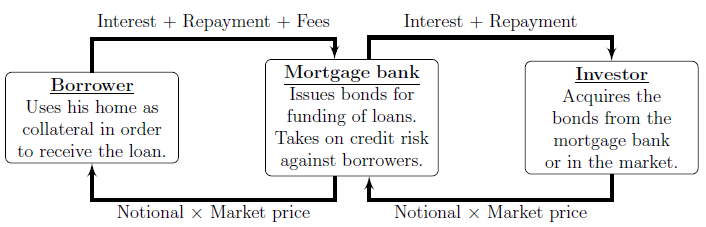
\includegraphics[width=1\linewidth]{figure/bond_cash_flow_illustration_23012022} 

}

\caption{Simplified illustration of the relationships and payment streams between the homeowner, the mortgage bank and the investor in the Danish mortgage system.}\label{fig:bondCashFlow}
\end{figure}
To understand why the Danish mortgage system is of interest is due to impact on
the Danish economy and the significant size of the market, being the largest covered
bond market in Europe (ECBC 2021), where in December 2021 the Danish mortgage market amounted to DKK 3,177 billions.

According to the Danish central bank, Nationalization, the foreign ownership of Danish Mortgage bonds totalled DKK 802 billions as of Dec 2021 or equivalent to 24\% of the total amount outstanding in the Danish mortgage system.

THe market for Danish mortgage bonds consits mainly of fixed coupon callable bonds, adjustable rate mortgage bonds and capped floating rate bonds.

The focus of this thesis will be on the fixed income coupon callable bonds due it being the most complex of the aforementioned.,

In order to understand the different aspects of a callable bond, we will first have to introduce the term structure theory and build a framework for descrying the behaviour of the yield curve. This in done in \ref{theory}

\hypertarget{the-danish-mortgage-market}{%
\chapter{The Danish Mortgage Market}\label{the-danish-mortgage-market}}

Being one of the oldest and most stable bond markets in the world, the Danish Bond market has it's root all the way back to 1797 where the first mortgage bank Kreditkassen for Husejere i Kjøbenhavn was established to help rebuild Copenhagen after the devastating fire of 1795 where a quarter of the city was lost to the fire.

The objective of stabilibty can also be seen in the resistance of the Danish Mortgage Market to economic crises, as the Danish economy has gone through several crises the past 50 years.
\begin{itemize}
\tightlist
\item
  The two oil crises of the 1970's
\item
  The 1986 austerity package and the 1987 tax reform
\item
  The Dot-com bubble in 2000
\item
  The financial crises
\end{itemize}
Arguable each crises has had an effect on the mortgage system differently and have even caused substitutional losses to the mortgage banks. However the losses have never affected the investors, as not one Danish Mortgage bondholder has lost the investment or even part of it. Moreover, the market stayed active and liquid under the financial crisis as evidenced by (Dick-Nielsen, Feldhütter, and Lando 2012; Gundersen, Hesselberg, and Hove 2011), where both find that the Danish Mortgage Bonds were as liqui as the Danish Government bonds during years from 2008 to 2009.

\hypertarget{types-of-mortgage-bonds}{%
\section{Types of mortgage bonds}\label{types-of-mortgage-bonds}}

The Danish mortgage market mainly consists of the following types of mortgage bonds
\begin{itemize}
\item
  ARMs - Adjustable Rate Mortgage Securities. which are subject to refinancing until the longer-term underlying loan has matured. The maturities match the fixed-rate period of the underlying loan, and are mainly 1 to 5 yers and the bond type is bullet
\item
  Floating-rate note - Variable-rate annuities with redemptions matching the underlying loans. The maturites mainly range from 1 to 5 years.
\item
  Capped floater - Variable-rate annuities with redemptions not matching the underlying loans. The maturites are mainly from 5 to 30 years
\item
  Callable bonds - Fixed rate callable annuities, where payments and redemptions match the underlying loan. The maturities are mainly 15, 20 or 30 years.
\end{itemize}
All 4 types of mortgage bonds have underlying loans where maturires of up to 30 years are available. Furthermore, most loans can be offered with an interest only(IO) period up to 30 years. If the IO option is chosen, the loan must be repaid as an bullet bond at maturity, otherwise if a IO period of 10 years is chosen, the loan must be repaid as an annuity profile for the remaining lifetime of the loan i.e.~20 years. In recent years the amount of loans with interest only option has declined and as of December 2021, interest only loans accounts for 43.5 \%\footnote{Nationalbanken Statistics - DNRUDDKI} of the loans to Danish house-holds.

\hypertarget{the-danish-mortgage-model}{%
\section{The Danish mortgage model}\label{the-danish-mortgage-model}}

The Danish mortgage model is based upon a stable and transparent system, with several advantages and unique features. Since mortgage banks does not function as commercial banks, and only able to fund loans through the sale of bonds which limits the risk of the mortgage banks Hence, the mortgage bank protects the investor from borrower defaulting. The mortgage bank secures the issued bond by using the cover pool which consist of collateral in terms of the claims against the borrows as well as additional securities posed by the mortgage bank to protect the investor from losses. These securities constitute what is known as overcollateralization and should be of very high credit quality.

\hypertarget{match-funding-principle}{%
\section{Match funding principle}\label{match-funding-principle}}

The match-funding principle entails that for every loan made by the mortgage bank, a new bond is issued with matching cash-flow properties. This eliminates mismatch in cash-flows and refinancing risk for the mortgage bank, which also secures payments to the bondholder. In the Danish mortgage system the mortgage bank functions as an intermediary between the investor and the borrower. Mortgage banks funds loans on a current basis, meaning that hte bond must be sold before the loan can be given. This also entails that the market price of the bond determines the loan rate. THe loan is therefore equal to the investment, which passes through the mortgage bank. Repayment and interest from the borrower to investor also passed through them mortgage bank, however the mortgage bank changes the borrower a margin though the lifetime of the loan, which is a percentage of the debt outstanding.

Since mortgage banks is only an intermediary it is not affected by changes in the floating rate, as it passes repayments and interest through to the investor. The drawback for the mortgage bank is that it endures the credit risk in the event of a default of the borrower, as it still has to make repayment and interest to the bond holder. This however protects the investor as the credit risk is removed, but is also a great incentive for the mortgage bank to put an emphasis on the due diligence process when issuing loans and adds to the stability of the system. Part of the due diligence is not only the valuing the property when making a credit assessment of a potential borrower, but also assessing the borrower's current economic situation including income and wealth based on legislation that dictates eligibility for granting and funding loans.

\hypertarget{delivery-and-prepayment}{%
\section{Delivery and prepayment}\label{delivery-and-prepayment}}

A central unique feature of the Danish mortgage model is the delivery option which means that the borrower always ahs the possibility of buying the underlying bond in the market, and delivering it back to the mortgage bank, which then cancels the loan. This is unique way for the borrower to reduce the notional amount of the loan if interest rate rises, and the related bond price falls. It is also a hedging effect on the expected drop in house prices that follows increasing interest rates as the two effect offset each other. This has no effect on the investor in terms of payments made from the investors to the bondholders.

Callables bonds also have a prepayment option( embedded call-option). The prepayment option gives the borrower the opportunity to repay the loan at pari (100) at every quarter throughout the lifetime of the loan.

Capped floaters have a similar prepayment option, however the prices depends on the contract is typically 105. This is favorable when the current available coupon rate is below the coupon rate on the mortgage.

The prepayment on Danish callables and capped floaters are more difficult to price than corresponding bond without the prepayment option and come with an additional option and come with an additional prepayment risk for the investor, this is however compensated with a higher interest rate.

The prepayment risk arises from the option to prepay the loan at pari, which exposes the investor to the risk of not being able to reinvest at the same conditions. The rational scenarios for prepayment are depicted in figure \ref{fig:prepayment}
\begin{figure}

{\centering \includegraphics[width=1\linewidth]{figure/prepay} 

}

\caption{Pricing curve of Callabalbe Bonds and Non-callable bonds.}\label{fig:prepayment}
\end{figure}
When prices are close to par the price of the callable bond is lower than the price of a non-callable bond, i.e.~government bond, as the chance of prepayment increases. However the borrowers are not always rational, which can create opportunities for the active investor, but is also a source of risk for a buy-and-hold strategy.

\hypertarget{prepayment-risk}{%
\section{Prepayment Risk}\label{prepayment-risk}}

The borrowers have the possibility to repay (part of) the notional before maturity, these kinds of anticipated and unexpected payments are called prepayment. this make the duration of the mortgage bond stochastic, which creates complication in refinancing for the investor. The investor is interested in prepayment rate on a security level, rather than a single borrower.\\
A prepayment option is an option which ``reflect the difference between the value of the outstanding loan repayments at the interest rate at the time of the prepayment for the remaining term of the loan minus the amount of the loan then outstanding (which is the value of the outstanding loan repayments at the original loan interest rate) (SHERRIS 1994).\\
if the interest rate goes down then the option is in the money, controversially if the interest rate goes up the optionality is out of the money. The exercise price of this call is equal to the loan outstanding. Rationally, the call should be exercised only if the difference mentioned above is positive since, otherwise, the option is worth more if you don't exercise it. Meaning thta it is more convenient to put money in a saving account rather than prepay the mortgage. However borrowers does not always act economically rational though, from now on we will use the the term non-ration to identify something that differs from the economically rational behaviour explained earlier.

An American call option on an amortizing reducing term swap could be a good instrument to hedge the prepayment option, but the ideal hedge instrument may not exist. For instance, assuming that the duration on the financing and of the loan are perfectly matched, suppose a 20 years mortgage loan at 4\% is financed with a 20 years bond paying 3.5 \%. If the interest rate goes down to 3\%, the borrower will have to refinance at the new rate prepaying the old mortgage and opening a new one at the lower interest rate. However, the bank will still have the obligation of paying 3.5 \% interest on the bond used to finance the first loan. Moreover, since the price of the perfect hedge instrument is equal to the cost of the prepayment option., if this instrument existed, it could be use to price the option (SHERRIS 1994).

The possibility to prepay exposes the bank to prepayment risk, which can be divided in two classes (Consalvi and Freca 2010)
\begin{itemize}
\item
  Interest rate risk - This arises because fixed rate mortgage are hedged against interest rate change using Interest Rate Swaps (IRS). The bank receives the floating rate and pays the fixed one, this means that a prepayment may expose the bank to the possibility of paying a fixed rate on the derivative which is higher than the one obatined on the new loans.
\item
  Liquidity risk - Arises from the fact that the liquidity profile of the bank is strongly influence by the maturity profile of the mortgage conditional to prepayments. An incorrect estimation of this quantity leads to the risk of under or over funding and of higher long-term liquidity costs.
\end{itemize}
Since prepayment are substation risk for the investor, is is fundamental to be able to predict the conditional prepayment rate (CPR), which is the proportion of the pricing of a pool of loans assumed to prepay in each period, in order to better forecast future cash flows.\\
When modelling mortgage prepayment, we cannot just use the rational assumption as mentioned earlier to evaluate contracts (e.g.~prepay only when the interest rate goes down), but we have to take into account the behaviour aspect as well, and hence we need to have a behavioural approach. In such a model we take into account factors usually estimated through statical analysis, in order to explain effect that otherwise could not have been explained. These kinds of techniques are called exogenous models, in opposition to optional prepayment models that see prepayment just as a consequence of rational behaviour e.g prepayment is always exercised at an optimal time by the borrower.\\
For these reason, rather than using a rational prepayment model for which the prepayment rate depends on just the rate evolution, an empirical model which is capable of taking into account other factors is chosen. This CPR is a function of some variable like the refinance incentive, the seasoning, the age of the loan, etc,

\hypertarget{incentives-to-prepay}{%
\section{Incentives to prepay}\label{incentives-to-prepay}}

\hypertarget{theory}{%
\chapter{Theory}\label{theory}}

\hypertarget{term-strucutre}{%
\section{Term Strucutre}\label{term-strucutre}}

\hypertarget{callable-mortgage-bonds}{%
\section{Callable Mortgage Bonds}\label{callable-mortgage-bonds}}

\hypertarget{estimating-prepayments-application-of-machine-learning}{%
\section{Estimating prepayments, application of machine learning}\label{estimating-prepayments-application-of-machine-learning}}

\hypertarget{ke}{%
\section{Ke}\label{ke}}

\hypertarget{data}{%
\chapter{Data}\label{data}}

\hypertarget{estimation}{%
\chapter{Estimation}\label{estimation}}

\hypertarget{discussion}{%
\chapter*{Discussion}\label{discussion}}
\addcontentsline{toc}{chapter}{Discussion}

\hypertarget{conclusion}{%
\chapter*{Conclusion}\label{conclusion}}
\addcontentsline{toc}{chapter}{Conclusion}

\appendix

\hypertarget{the-first-appendix}{%
\chapter{The First Appendix}\label{the-first-appendix}}

This first appendix includes all of the R chunks of code that were hidden throughout the document (using the \texttt{include\ =\ FALSE} chunk tag) to help with readibility and/or setup.

\textbf{In the main Rmd file}
\begin{Shaded}
\begin{Highlighting}[]
\CommentTok{\# This chunk ensures that the thesisdown package is}
\CommentTok{\# installed and loaded. This thesisdown package includes}
\CommentTok{\# the template files for the thesis.}
\ControlFlowTok{if}\NormalTok{ (}\SpecialCharTok{!}\FunctionTok{require}\NormalTok{(remotes)) \{}
  \ControlFlowTok{if}\NormalTok{ (params}\SpecialCharTok{$}\StringTok{\textasciigrave{}}\AttributeTok{Install needed packages for \{thesisdown\}}\StringTok{\textasciigrave{}}\NormalTok{) \{}
    \FunctionTok{install.packages}\NormalTok{(}\StringTok{"remotes"}\NormalTok{, }\AttributeTok{repos =} \StringTok{"https://cran.rstudio.com"}\NormalTok{)}
\NormalTok{  \} }\ControlFlowTok{else}\NormalTok{ \{}
    \FunctionTok{stop}\NormalTok{(}
      \FunctionTok{paste}\NormalTok{(}\StringTok{\textquotesingle{}You need to run install.packages("remotes")",}
\StringTok{            "first in the Console.\textquotesingle{}}\NormalTok{)}
\NormalTok{    )}
\NormalTok{  \}}
\NormalTok{\}}
\ControlFlowTok{if}\NormalTok{ (}\SpecialCharTok{!}\FunctionTok{require}\NormalTok{(thesisdown)) \{}
  \ControlFlowTok{if}\NormalTok{ (params}\SpecialCharTok{$}\StringTok{\textasciigrave{}}\AttributeTok{Install needed packages for \{thesisdown\}}\StringTok{\textasciigrave{}}\NormalTok{) \{}
\NormalTok{    remotes}\SpecialCharTok{::}\FunctionTok{install\_github}\NormalTok{(}\StringTok{"ismayc/thesisdown"}\NormalTok{)}
\NormalTok{  \} }\ControlFlowTok{else}\NormalTok{ \{}
    \FunctionTok{stop}\NormalTok{(}
      \FunctionTok{paste}\NormalTok{(}
        \StringTok{"You need to run"}\NormalTok{,}
        \StringTok{\textquotesingle{}remotes::install\_github("ismayc/thesisdown")\textquotesingle{}}\NormalTok{,}
        \StringTok{"first in the Console."}
\NormalTok{      )}
\NormalTok{    )}
\NormalTok{  \}}
\NormalTok{\}}
\FunctionTok{library}\NormalTok{(thesisdown)}
\CommentTok{\# Set how wide the R output will go}
\FunctionTok{options}\NormalTok{(}\AttributeTok{width =} \DecValTok{70}\NormalTok{)}
\end{Highlighting}
\end{Shaded}
\textbf{In Chapter \ref{ref-labels}:}

\hypertarget{roadmap}{%
\chapter*{Roadmap}\label{roadmap}}
\addcontentsline{toc}{chapter}{Roadmap}

\hypertarget{timeline}{%
\section*{Timeline}\label{timeline}}
\addcontentsline{toc}{section}{Timeline}

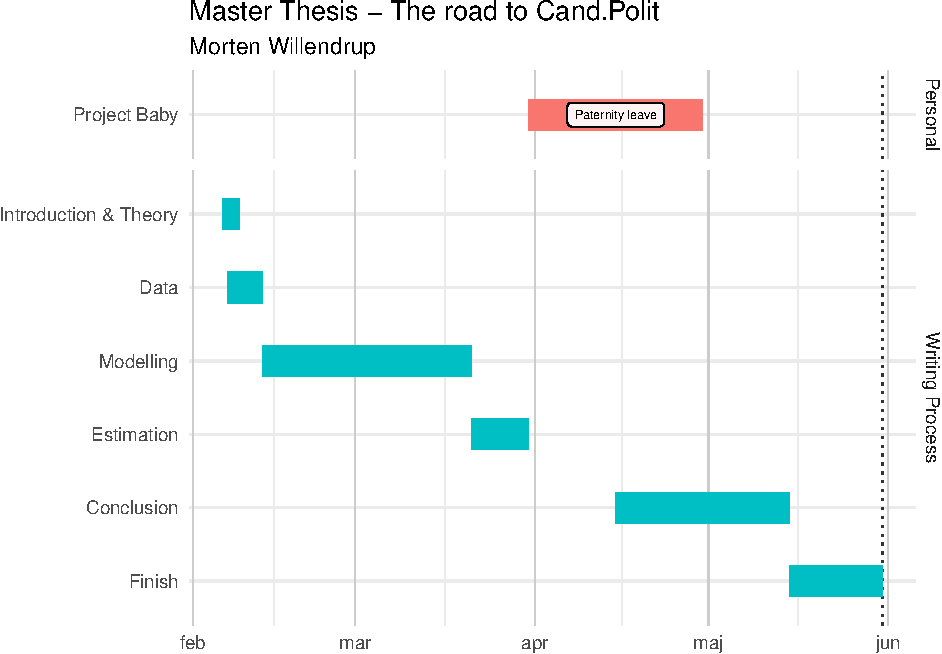
\includegraphics{thesis_files/figure-latex/roadmap-1.pdf}

\hypertarget{introduction}{%
\section*{Introduction}\label{introduction}}
\addcontentsline{toc}{section}{Introduction}

Need to write a full introduction of the Danish Mortgage Market, furthermore
leave space for a brief walkthorugh of the thesis

\hypertarget{theory-1}{%
\section*{Theory}\label{theory-1}}
\addcontentsline{toc}{section}{Theory}

Relevant theory should be Machine Learning, which is relevent should be discussed
in detail

\hypertarget{data-1}{%
\section*{Data}\label{data-1}}
\addcontentsline{toc}{section}{Data}

Get data from DST.\\
Get data from Nasdaq.\\
Get data from Danske Bank Asset Management

\backmatter

\hypertarget{references}{%
\chapter*{References}\label{references}}
\addcontentsline{toc}{chapter}{References}

\markboth{References}{References}

\noindent

\setlength{\parindent}{-0.20in}

\hypertarget{refs}{}
\begin{CSLReferences}{1}{0}
\leavevmode\vadjust pre{\hypertarget{ref-angel2000}{}}%
Angel, Edward. 2000. \emph{Interactive Computer Graphics : A Top-down Approach with OpenGL}. Boston, MA: Addison Wesley Longman.

\leavevmode\vadjust pre{\hypertarget{ref-angel2001}{}}%
---------. 2001a. \emph{Batch-File Computer Graphics : A Bottom-up Approach with QuickTime}. Boston, MA: Wesley Addison Longman.

\leavevmode\vadjust pre{\hypertarget{ref-angel2002a}{}}%
---------. 2001b. \emph{Test Second Book by Angel}. Boston, MA: Wesley Addison Longman.

\leavevmode\vadjust pre{\hypertarget{ref-consalvi2010measuring}{}}%
Consalvi, Matteo, and G Scotto di Freca. 2010. {``Measuring Prepayment Risk: An Application to UniCredit Family Financing.''} \emph{UniCredit and Universities, Working Paper}.

\leavevmode\vadjust pre{\hypertarget{ref-dick2012corporate}{}}%
Dick-Nielsen, Jens, Peter Feldhütter, and David Lando. 2012. {``Corporate Bond Liquidity Before and After the Onset of the Subprime Crisis.''} \emph{Journal of Financial Economics} 103 (3). Elsevier: 471--92.

\leavevmode\vadjust pre{\hypertarget{ref-ECBC2021}{}}%
ECBC. 2021. {``European Covered Bond Fact Bbook 2021.''} \url{https://hypo.org/app/uploads/sites/3/2021/09/ECBC-Fact-Book-2021-FINAL.pdf}.

\leavevmode\vadjust pre{\hypertarget{ref-Gundersen2011}{}}%
Gundersen, Poul, Stig Hesselberg, and Sean Hove. 2011. {``Danish Mortgage Credit.''} \emph{Monetary Review}. Nationalbanken.

\leavevmode\vadjust pre{\hypertarget{ref-jensen2013rentesregning}{}}%
Jensen, Bjarne Astrup. 2013. \emph{Rentesregning: S{æ}rtryk Af 6. Udgave}. Dj{ø}f Forlag.

\leavevmode\vadjust pre{\hypertarget{ref-sherris1994pricing}{}}%
SHERRIS, MICHAEL. 1994. {``Pricing and Hedging Loan Prepayment Risk.''} \emph{Transactions of Society of Actuaries}.

\end{CSLReferences}

% Index?

\end{document}
